\documentclass[12pt]{article}

\newcommand{\project}[1]{\textsl{#1}}
\newcommand{\foreign}[1]{\textsl{#1}}
\newcommand{\etal}{\foreign{et~al.}}

\newcommand{\given}{\,|\,}
\newcommand{\dd}{\mathrm{d}}
\newcommand{\setofall}[1]{\left\{{#1}\right\}}
\renewcommand{\star}{\mathrm{star}}
\newcommand{\galaxy}{\mathrm{gal}}
\newcommand{\quasar}{\mathrm{qso}}
\newcommand{\mml}{\mathrm{MML}}

\usepackage[]{graphicx}
\usepackage[]{subcaption}
\usepackage{float}

\title{Hierarchical probabilistic point-source classification for SDSS Stripe 82}
\author{some mix of Bochanski, Fadely, Hogg, Preston, Willman, and others}
\date{DRAFT VERSION 2012-10}

\begin{document}
\maketitle

\begin{abstract}
Ground-based optical studies of the Milky Way face the challenge that
at faint magnitudes, galaxies are not cleanly distinguishable from
stars on morphological grounds alone.  This problem is especially
severe at magnitudes at which galaxies enormously outnumber stars.
Fortunately, these surveys tend to be multi-band and the photometry
usually comes with reasonable uncertainty estimates.  Here we use an
unsupervised, template-based hierarchical Bayesian model to capitalize
on multi-band photometry to classify angularly compact sources into
star, galaxy, and quasar classes.  We apply the method to the
\project{Sloan Digital Sky Survey Stripe 82} imaging data set.  We
find XXX and YYY.  All our code and all of its output on the
\project{Stripe 82} data are available at ZZZ.
\end{abstract}

\section{Introduction}

Start with the ratios of stars, galaxies and quasars as a function of
apparent magnitude, color, and angular size cut.  This could be a
paper on its own!

Hogg to Beth: One way to think about this problem is as a data
imputation problem: Can we accurately predict the high-resolution
(say, \project{HST}-resolution) size measurement using the multi-band
low-resolution (ground-based) photometric measurements, in which the
source is unresolved?

Most approaches to this problem are supervised approaches.  These are
bad because test data (the new data of interest) are never
statistically like training data (previous-generation data no longer
of interest).

In previous work (Fadely \etal\ 2012) we have shown that an
unsupervised hierarchical Bayesian methodology outperforms the best
supervised classification methods in the realistic situations in which
we find ourselves: We have a good noise model for our data, but we
don't have training data at the same depth or signal-to-noise as the
test data (data of interest).

\section{Method}

\begin{eqnarray}
p(d_i\given j,C_{ij},I) &=& A_i\,\exp(-\frac{1}{2}\,\chi^2_{ij})
\\
p(d_i\given j,I) &=& \int p(d_i\given j,C_{ij},I)\,p(C_{ij}\given I)\,\dd C_{ij}
\\
p(d_i\given \star,I) &=& \sum_j p(d_i\given j,I)\,P(j\given I)
\\
p(d_i\given I) &=& \sum_{q\in\setofall{\star,\galaxy,\quasar}} p(d_i\given q,I)\,P(q\given I)
\\
p(\setofall{d_i}_i\given I) &=& \prod_i p(d_i\given I)
\\
I_{\mml} &\leftarrow& \arg\max_I p(d_i\given I)
\\
p(\star\given d_i,I_{\mml}) &=& \frac{1}{Z_i}\,p(d_i\given \star,I_{\mml})\,P(\star\given I_{\mml})
\\
Z_i &\equiv& p(d_i\given I_{\mml})
\quad ,
\end{eqnarray}
where $I$ represents all the assumptions and hyper-parameters and
$I_{\mml}$ is the maximum-marginalized likelihood values for all those
assumptions and hyperparameters (that we permitted to vary).  This
method is called ``empirical Bayes'', apparently.

Beth question: Are the posterior probabilities true probabilities?
Hogg answer: Yes, but conditional on some hella unrealistic
assumptions.

\section{Data}
We obtained data for 217578 Stripe 82 sources by running a clean photometry query on the Stripe 82 database of the \project{SDSS} Catalog Archive Server. This query was modified from (Annis et al.) to select only sources in the RA and dec range of the VIMOS VLT Deep Survey (\project{VVDS}), with the goal of using VVDS spectroscopic information to test the performance of our star-galaxy separation in Stripe 82. 

Of these Stripe 82 objects, 23\% are defined as point sources with $|r_{\mathrm{psf}} - r_{\mathrm{model}}| < 0.03$ (Annis et al.).  We matched all sources to the VVDS data with a match radius of $0.00055^\circ $ $(1.98^{\prime\prime})$. (beth: where did VVDS data come from?) The resulting match list includes 13105 sources; 5581 are stars according to \project{VVDS} $(z = 0.0)$, and 7524 are galaxies $(z > 0.0)$. The locations of the Stripe 82 data and VVDS matches in color-magnitude space are compared in Figure \ref{cmd}.

In order to compare the performance of the morphological separator in the coadd to that in the single pass \project{SDSS} catalog, we also matched \project{SDSS DR7} data to \project{VVDS} sources using the same query and matching procedure. This resulted in 12335 matched sources, of which 5922 are stars and 6413 are galaxies.

\begin{figure}[h!]
	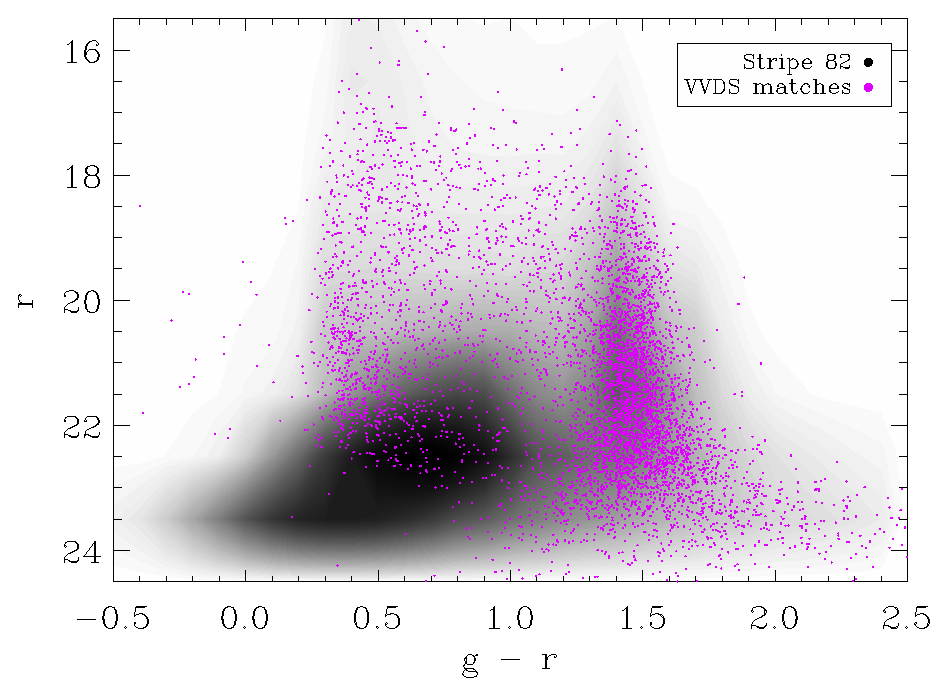
\includegraphics[width=0.8\textwidth]{final_figures/cmd.eps}
	\caption{Color-magnitude diagram of Stripe 82 sources within the range of \project{VVDS}, $333.2 < \mathrm{RA} < 335.6$ and $-0.51 < \mathrm{dec} < 1.25$, with matched sources highlighted. The overlap is focused on the redder sources in Stripe 82, while the locus of bluer objects largely does not correspond to sources in \project{VVDS}.}
	\label{cmd}
\end{figure}

(...Discussion of \project{SDSS} star--galaxy separators in common use.)

\project{SDSS} defines stars as objects for which $|r_{\mathrm{psf}} - r_{\mathrm{model}}| \leq 0.145$ (Abazajian et al. 2004). Because this cutoff misclassifies many faint galaxies as stars in the coadded data, (Annis et al.) use the stricter criterion $|r_{\mathrm{psf}} - r_{\mathrm{model}}| \leq 0.03$ for Stripe 82 (see Figure \ref{morph}. At $r = 20$, 96.7\% of single pass and 92.9\% of coadd sources in the matched catalog are classified correctly using these cutoffs. However, the accuracy of these criteria varies significantly as a function of magnitude, especially when considering both the purity and completeness for stars and galaxies separately (see Figure \ref{cp}). Adjusting the cutoff can improve performance in some areas, but there is no $|r_{\mathrm{psf}} - r_{\mathrm{model}}|$ cutoff for either single pass or coadded data that optimizes both purity and completeness for stars and galaxies (see Figure \ref{cutoff}).

\begin{figure}[h!]
	\centering
	\begin{subfigure}[]{0.8\textwidth}
		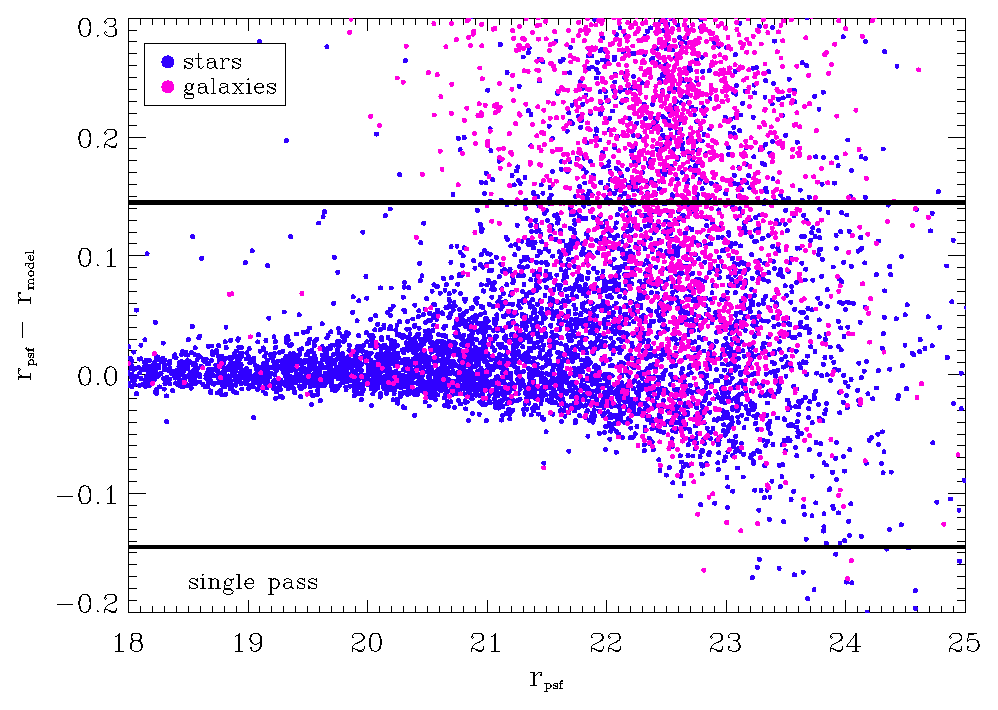
\includegraphics[width=\textwidth]{final_figures/singlepass_morph.eps}
	\end{subfigure}
	\begin{subfigure}[]{0.8\textwidth}
		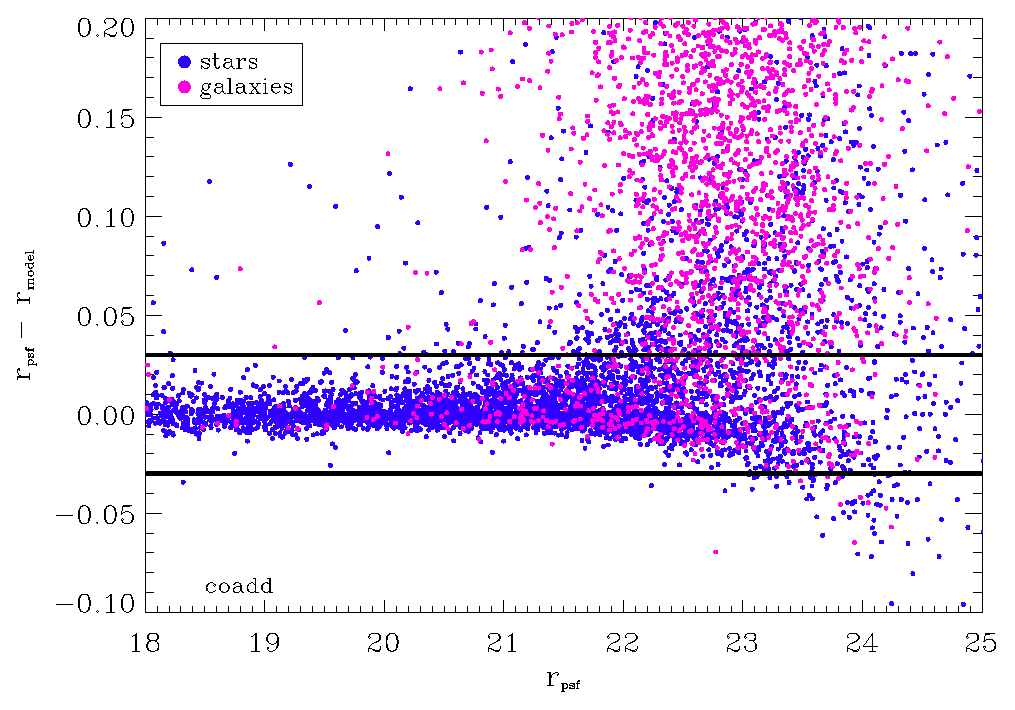
\includegraphics[width=\textwidth]{final_figures/coadd_morph.eps}
	\end{subfigure}
	\caption{Stripe 82 sources with matches in \project{VVDS}, categorized by their \project{VVDS} classification ($z = 0.0$ for stars). Single pass data are shown with the standard \project{SDSS} star/galaxy separation cutoff, $| r_{\mathrm{psf}} - r_{\mathrm{model}} | < 0.145$; coadd data are shown with the morphological cutoff used in (Annis et al), $| r_{\mathrm{psf}} - r_{\mathrm{model}} | < 0.03$. The clear stellar locus becomes much less apparent at faint magnitudes.}
	\label{morph}
\end{figure}

\begin{figure}[h!]
	\centering
	\begin{subfigure}[]{0.49\textwidth}
		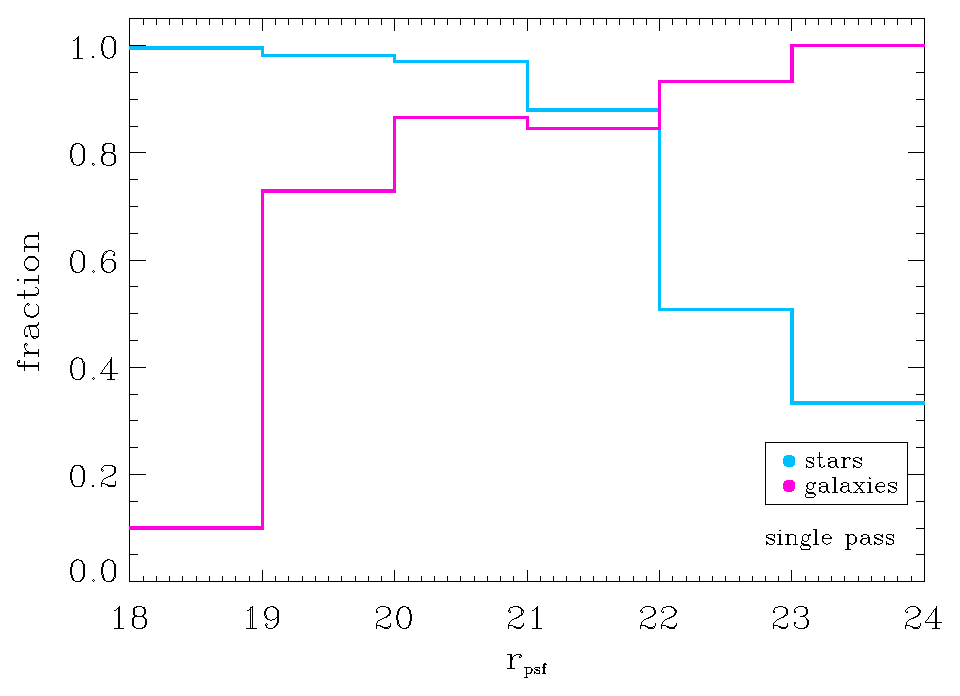
\includegraphics[width=\textwidth]{final_figures/singlepass_completeness.eps}
	\end{subfigure}
	\begin{subfigure}[]{0.49\textwidth}
		\includegraphics[width=\textwidth]{final_figures/singlepass_purity.eps}
	\end{subfigure}
	
	\begin{subfigure}[]{0.49\textwidth}
		\includegraphics[width=\textwidth]{final_figures/coadd_completeness.eps}
		\caption{Completeness}
	\end{subfigure}
	\begin{subfigure}[]{0.49\textwidth}
		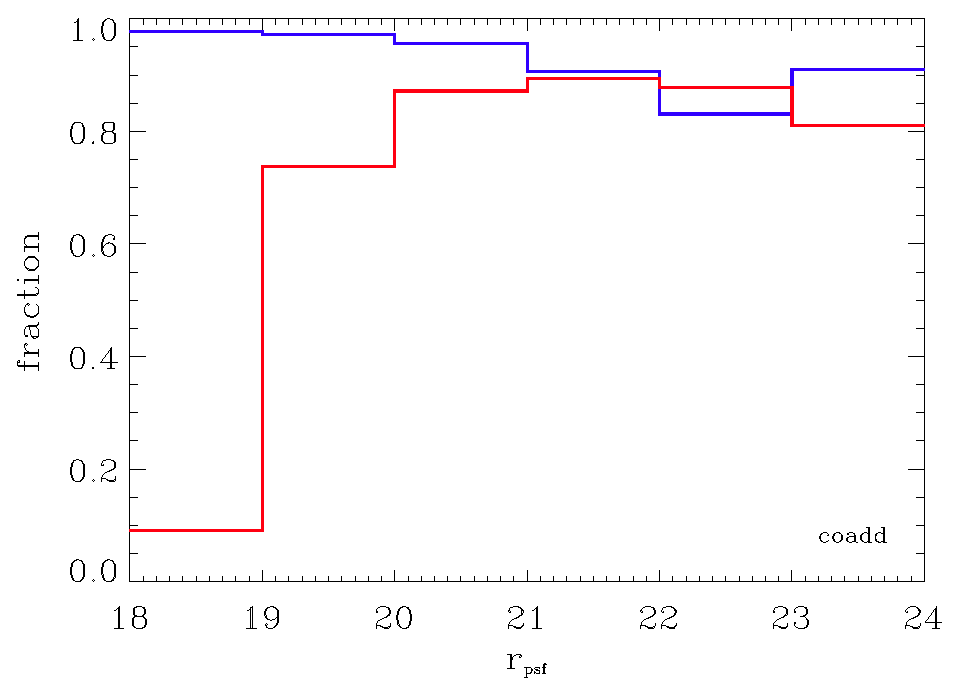
\includegraphics[width=\textwidth]{final_figures/coadd_purity.eps}
		\caption{Purity}
	\end{subfigure}
	\caption{Completeness (e.g., the fraction of stars that are classified as stars) and purity (e.g., the fraction of objects classified as stars that are stars) as a function of  $r_{\mathrm{psf}}$ magnitude for single pass and coadd data. At fainter magnitudes, the morphological separators misclassify many stars as galaxies.}
	\label{cp}
\end{figure}

\begin{figure}[h!]
	\begin{subfigure}[h]{0.7\textwidth}
		\includegraphics[width=\textwidth]{final_figures/singlepass_cutoff.eps}
	\end{subfigure}
	
	\begin{subfigure}[h]{0.7\textwidth}
		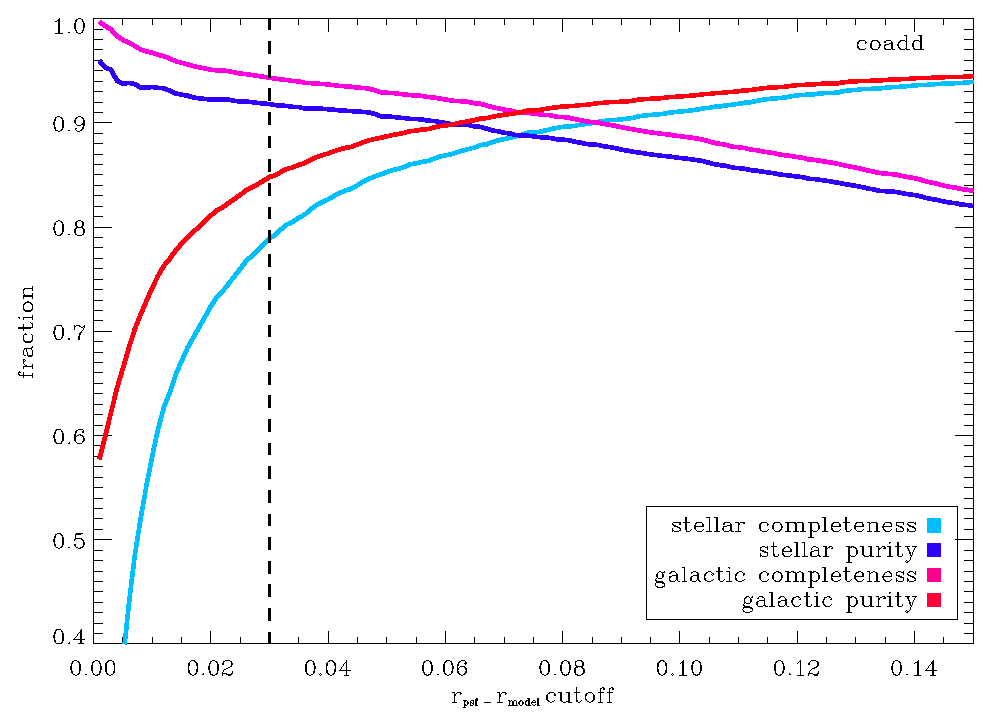
\includegraphics[width=\textwidth]{final_figures/coadd_cutoff.eps}
	\end{subfigure}
	\caption{Completeness and purity for stars and galaxies as a function of morphological separation cutoff. Varying the $|r_{\mathrm{psf}} - r_{\mathrm{model}}|$ cutoffs would improve the separators' performance in some areas while diminishing it in others.}
	\label{cutoff}
\end{figure}

\section{Results}
Matching Stripe 82 sources to the \project{VVDS} catalog allows us to compare our classifications with spectroscopic classifications for corresponding \project{VVDS} sources. The usefulness of this method depends upon the reliability of the matches found. The primary feature in Figure \ref{morph} that arouses suspicion of the robustness of the matches is the presence of several galaxies in the bright portion of the defined stellar locus...(looking into this more)

*discrepancy in demographics between Stripe 82 and \project{VVDS}

How are we going to test the results?  One option is to go to sources
covered by \project{HST} pointings and plot the \project{HST}-measured
size against each of several star--galaxy separation variables,
including likelihood ratios, posterior probabilities, SVM boundary
distances, psf-minus-model magnitudes, and the like.

Bochanski went through and grabbed a bunch of Sextractor source lists
from ACS, WFC3 and WFPC2 images from the HLA.

VVDS and PRIMUS have unbiased spectroscopic databases that would be
useful for testing the star--galaxy separators. 

Another more speculative is to see if we can see significance of some
\project{Stripe 82} stellar structure rise as we apply our method.

Another is to see if we predict photometric bands or colors \emph{not}
used in the HB inference.  That would be a ``posterior predictive
check'' which is not \emph{directly} relevant, but should correlate
with performance.

\section{Discussion}

What worked, what didn't?

What approximations did we make and how are they likely to be hurting
us?

What advice do we have for just-starting projects like \project{Dark
  Energy Survey}?  And of course \project{LSST}.

\end{document}
